\section[VAN]{VAN}
	\begin{equation}
	\label{eq:van}
	\begin{split}
 		w = - C_0 + \sum_{k=1}^n \frac{CF_k}{(1+r)^k}
	\end{split}
	\end{equation}
	Consideriamo, quindi, il valore del \ac{VAN} su $12$ flussi di cassa (\textit{cashflow}), corrispondenti alle stime sull'utile realizzato alla fine di ogni mese ed un \textbf{tasso di sconto} $r$ pari al \textbf{\ac{WACC}} (\ref{eq:wacc_tax_value}).\newline
	La formula (\ref{eq:van}) diventa, quindi:	
	\begin{equation}
	\label{eq:van_caso_studio}
	\begin{split}
 		w = - C_0 + \sum_{k=1}^{12} \frac{CF_k}{(1+0,01726)^k}
	\end{split}
	\end{equation}	
	Il valore $C_0$ corrisponde all'investimento iniziale del nostro progetto, quindi, pari al \textbf{CAPEX} $ 56\thinspace 170,20 \: \mbox{\euro}$.
	Assumiamo, inoltre, che i flussi mensili siano costanti nell'arco di un anno, quindi la quantità $CF_k$ non è più legata al k-esimo mese, si può esprimere, quindi, come $CF$:
	\begin{equation}
	\label{eq:flussi_cassa_mensili}
	\begin{split}
 		CF = x \:(fatturato \: mensile) - 60\thinspace 131,27 \: (OPEX)
	\end{split}
	\end{equation}	  	
la (\ref{eq:van_caso_studio}) diventa (il VAN diventa funzione dei flussi di cassa lordi $x$ quindi $w = y(x)$):	
	\begin{eqnarray}
	\label{eq:van_caso_studio_2}
 		y(x) & = & - 56\thinspace 170,20 + \sum_{k=1}^{12} \frac{x - 60\thinspace 131,27}{(1+0,01726)^k} \nonumber \\
 		 & = & -56\thinspace 170,20 + (x - 60\thinspace 131,27) \cdot \underbrace{\sum_{k=1}^{12} \frac{1} {(1+0,01726)^{k}}}_{{}=10,7528} \nonumber \\
 		 & = & -56\thinspace 170,20 + (x - 60\thinspace 131,27) \cdot 10,7528 \nonumber \\
 		 & = & -702\thinspace 749,72 + 10,7528 \cdot x 		
	\end{eqnarray}  		

	\begin{comment}	
	ci possiamo, quindi, calcolare il valore del \ac{TIR} corrispondente. Per definizione il \ac{TIR} è pari a:
	\begin{equation}
	\label{eq:tir}
	\begin{split}
 		\sum_{k=0}^n \frac{C_k}{(1+i)^k} = 0
	\end{split}
	\end{equation}	 

	\end{comment}
 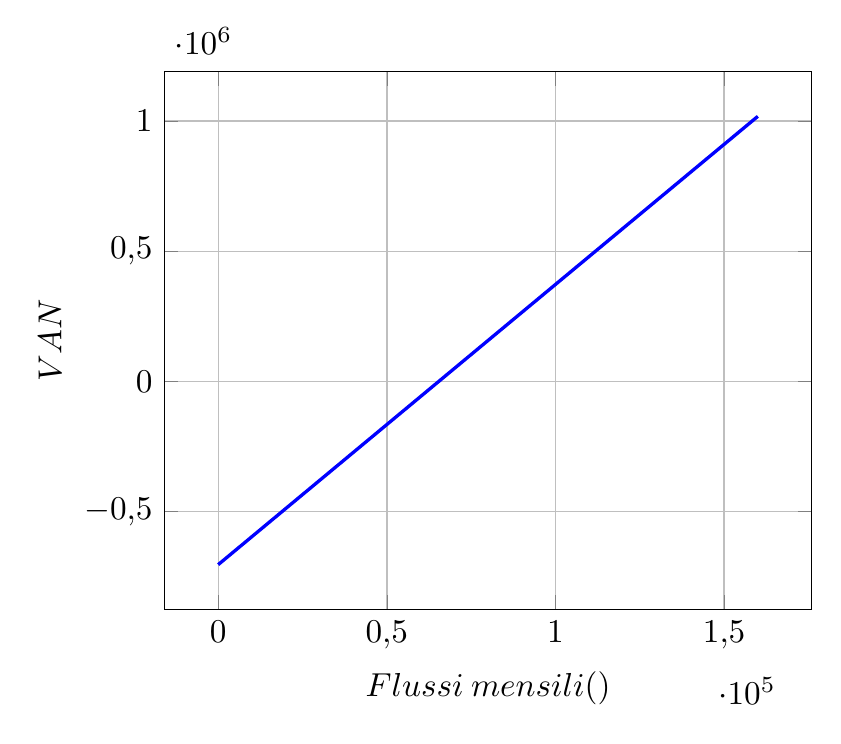
\begin{tikzpicture}[scale=1.2]
 \pgfkeys {
			/pgf/number format/.cd,
			set decimal separator={,{\!}},
			set thousands separator={}}
	\begin{axis}[ xlabel=$Flussi\: mensili (\mbox{\euro})$, 
				   ylabel=$VAN$, 
				   grid=major ]
		
		\addplot[domain=0:160000, color=blue, line width=1pt]{10.7528 * x - 702749.72};
		
	\end{axis}
\end{tikzpicture}

Un punto importante della funzione (\ref{eq:van_caso_studio_2}) è quello per cui il $ VAN = 0 $, ovvero:

	\begin{equation}
	\label{eq:van_zero}
	\begin{split}
 		y(x) = 0
 	\end{split}
	\end{equation}

Il valore $x$ per cui (\ref{eq:van_zero}) è soddisfatta 
	\begin{equation}
	\label{eq:van_pareggio_1}
	\begin{split}
 		10,7528 \cdot x - 702\thinspace 749,72 = 0	
 	\end{split}
	\end{equation}
è pari a:
	\begin{eqnarray}
	\label{eq:van_pareggio_2}
		x & = & \frac{702\thinspace 749,72	}{10,7528}	 	\nonumber \\[1.5ex] 
		  & = &  65\thinspace 355,04 \: \mbox{\euro} 
	\end{eqnarray}
Il valore di $x$ rappresenta, da un punto di vista fisico, il flusso minimo di cassa mensile affinchè il progetto risulti remunerativo alla fine del periodo in esame (12 mesi nel caso di studio proposto). \newline
Considerando il fatturato mensile pari a (\ref{eq:van_pareggio_2}), gli utili saranno pari a:
	\begin{equation}
	\label{eq:flussi_netti}
	\begin{split}
 		65\thinspace 355,04 \: \mbox{\euro} - \underbrace{60\thinspace 131,27 \: \mbox{\euro}}_{OPEX} = 5\thinspace 223,80 \: \mbox{\euro}	
 	\end{split}
	\end{equation}
fissando un tasso di sconto pari a (\ref{eq:wacc_tax_value}), si può osservare la seguente situazione:
%
%	Tabella relativa alla valutazione VAN = 0,00
%
\begin{savenotes}
\begin{table}[htb]
\centering
 \caption{VAN (Fatturato Mensile pari a $\mbox{\euro \:65\thinspace 355,04}$)}
 \begin{tabular}{p{5cm}D{,}{,}{7.2}D{,}{,}{7.2}D{,}{,}{7.2}}
 \toprule
 	\multicolumn{1}{c}{\textbf{Mese}} & \multicolumn{3}{c}{\textbf{Flussi di cassa (\euro)}} \\
 	& \multicolumn{1}{c}{Netti (\euro)} & \multicolumn{1}{c}{Attualizzati (\euro)} & \multicolumn{1}{c}{Totale (\euro)} \\
 \midrule
 	\makebox[5cm][r]{\textbf{Investimento Iniziale (CAPEX)}} & & & -56\thinspace 170,20 \\
 \midrule
 	\makebox[5cm][r]{Gennaio} & 5\thinspace 223,80 & 5\thinspace 134,97 & -51\thinspace 035,23\\ 
 	\makebox[5cm][r]{Febbraio} & 5\thinspace 223,80 & 5\thinspace 047,67 & -45\thinspace 987,59\\
 	\makebox[5cm][r]{Marzo} & 5\thinspace 223,80 & 4\thinspace 961,80 & -41\thinspace 025,79\\ 
 	\makebox[5cm][r]{Aprile} & 5\thinspace 223,80 & 4\thinspace 877,42 & -36\thinspace 148,37\\
 	\makebox[5cm][r]{Maggio} & 5\thinspace 223,80 & 4\thinspace 794,48 & -31\thinspace 353,89\\ 
 	\makebox[5cm][r]{Giugno} & 5\thinspace 223,80 & 4\thinspace 712,94 & -26\thinspace 640,95\\
 	\makebox[5cm][r]{Luglio} & 5\thinspace 223,80 & 4\thinspace 632,80 & -22\thinspace 008,15\\ 
 	\makebox[5cm][r]{Agosto} & 5\thinspace 223,80 & 4\thinspace 554,01 & -17\thinspace 454,14\\
 	\makebox[5cm][r]{Settembre} & 5\thinspace 223,80 & 4\thinspace 476,57 & -12\thinspace 977,57\\ 
 	\makebox[5cm][r]{Ottobre} & 5\thinspace 223,80 & 4\thinspace 400,44 & -8\thinspace 577,13\\
 	\makebox[5cm][r]{Novembre} & 5\thinspace 223,80 & 4\thinspace 325,61 & -4\thinspace 251,52\\ 
 	\makebox[5cm][r]{Dicembre} & 5\thinspace 223,80 & 4\thinspace 252,05 & 0,52\\ 
 	
 \bottomrule
 \end{tabular} 
\end{table}
\end{savenotes}
ovvero il 31 Dicembre i soci fondatori riescono a recuperare la somma investita il 1 Gennaio. 
Da un punto di vista grafico si osserva come il punto di coordinate \textbf{\textcolor{blue}{( 65355,04 ; 0 )}} rappresenti il \textit{punto di frontiera} tra due aree che presentano delle caratteristiche diverse, quella:
\begin{itemize}
\item \textbf{\color{red}{rossa}} è caratterizzata da tutti i flussi di cassa che \underline{non} permettono di rientrare dell'investimento ( pertanto il VAN è negativo );
\item \textbf{\color{green}{verde}} da tutti quei flussi per cui è possibile recuperare i CAPEX sostenuti all'avvio della società. Ovviamente maggiore saranno i flussi più breve risulterà il \textbf{periodo di pareggio}.
\end{itemize}

\usepgfplotslibrary{fillbetween}

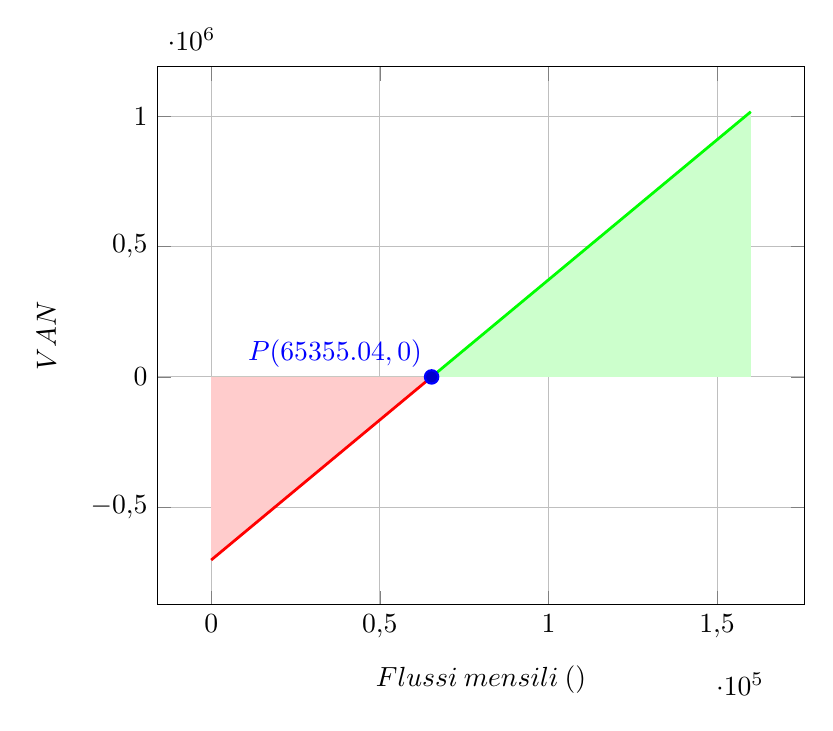
\begin{tikzpicture}[scale=1.2]
 \pgfkeys {
			/pgf/number format/.cd,
			set decimal separator={,{\!}},
			set thousands separator={}}

    \begin{axis}[thick,smooth, xlabel=$Flussi \: mensili \:(\mbox{\euro})$, ylabel=$VAN$, grid=major]    

		\addplot coordinates{( 65355.04, 0) };
							  
        \addplot+[domain=0:65355.04, name path=A,red,line width=1pt, no markers] {10.7528 * x - 702749.72};
        \addplot+[domain=65355.04:160000, name path=C,green,line width=1pt, no markers] {10.7528 * x - 702749.72};
        \addplot+[domain=0:160000, name path=B, draw=none,black, no markers] {0};

        \addplot[domain=0:65355.04, red!20] fill between[of=A and B];
        \addplot[domain=65355.04:160000, green!20] fill between[of=C and B];
        
        \coordinate[label=above left:\textcolor{blue}{$ P(65355.04,0)$}](a) at (65355.04,0);
    \end{axis}
\end{tikzpicture}
\newline
Da un punto di vista matematico, la (\ref{eq:van_caso_studio_2}) ammette come dominio tutto l'asse reale, ciò però \textit{fisicamente} non è possibile, perchè sarà vincolata \textit{a sinistra} dal valore del VAN in corrispondenza di $\mbox{\euro \: 0,00}$ flussi di entrate mensili (non è possibile avere entrate negative):  
	\begin{eqnarray}
	\label{eq:limite_sinistro}
 		y(0) & = & -702\thinspace 749,72 + 10,7528 \cdot 0 \nonumber \\
 								& = & -702\thinspace 749,72
	\end{eqnarray}
e come limite destro dal flusso di cassa mensile massimo raggiungibile $649\thinspace 001,60 \: \mbox{\euro}$ (corrispondenti a 8\thinspace 112,52 contratti):
	\begin{eqnarray}
	\label{eq:limite_superiore}
 		y(649\thinspace 001,60) & = & -702\thinspace 749,72 + 10,7528 \cdot 649\thinspace 001,60 \nonumber \\
 								& = & 6\thinspace 275\thinspace 834,68
	\end{eqnarray}
	
	\begin{tcolorbox}[colframe=blue!75!black,adjusted title=\textbf{Osservazione!}]
		Il \textbf{limite destro} è puramente teorico perchè si avrebbe nel caso in cui \underline{tutti} i potenziali clienti contattati stipulino alla fine il contratto del viaggio, situazione impossibile.
		\newline Il \textbf{limite sinistro}, invece, per quanto improbabile, può sempre verificarsi.
	\end{tcolorbox}	
in definitiva il dominio di (\ref{eq:van_caso_studio_2}) è pari a:
\[ Dom(y(x)) =	\left [ 0,00 ; 649\thinspace 001,60 \right)		\]
mentre il codominio di (\ref{eq:van_caso_studio_2}) è pari a:
\[ Codom(y(x)) =	\left [ -702\thinspace 749,72 ; 6\thinspace 275\thinspace 834,68 \right)		\]


%
%	Tabella relativa al caso teorico in cui non ci siano malati durante un anno
%
\begin{savenotes}
\begin{table}[htb]
\centering
 \caption{Variazione VAN}
 \begin{tabular}{p{3cm}D{,}{,}{5.2}D{,}{,}{5.2}D{,}{,}{5.2}D{,}{,}{7.4}}
 \toprule
 	& \multicolumn{1}{c}{Flusso di cassa mensile (\euro)} & \multicolumn{1}{c}{Contratti Mensili } &\multicolumn{1}{c}{\textbf{VAN}}&\multicolumn{1}{c}{\textbf{ \% Contratti}} \\
 \midrule	
	\makebox[3cm][r]{Ottimo} & 649\thinspace 001,60 & 8\thinspace 112,52 & 6\thinspace 275\thinspace 834,68 & 1,0000\\
 	\rowcolor[gray]{.7} \makebox[3cm][r]{Pareggio} & 65\thinspace 355,04 & 816,94 & 0,00 & 0,1007\\
 	\makebox[3cm][r]{Peggiore} &  0,00 & 0,00 & -702\thinspace 749,72 & 0,0000\\ 
 \bottomrule
 \end{tabular} 
\end{table}
\end{savenotes}

\subsection[Caso di Studio Realistico]{Caso di Studio Realistico}
\begin{savenotes}
\begin{table}[htb]
\centering
 \caption{Variazione VAN (Casi di Studio)}
 \begin{tabular}{p{3cm}D{,}{,}{5.2}D{,}{,}{5.2}D{,}{,}{5.2}D{,}{,}{7.4}}
 \toprule
 	& \multicolumn{1}{c}{Flusso di cassa mensile (\euro)} & \multicolumn{1}{c}{Contratti Mensili } &\multicolumn{1}{c}{\textbf{VAN}}&\multicolumn{1}{c}{\textbf{ \% Contratti}} \\
 \midrule	
	\makebox[3cm][r]{Ottimo} & 649\thinspace 001,60 & 8\thinspace 112,52 & 6\thinspace 275\thinspace 834,68 & 1,0000\\
	\makebox[3cm][r]{Caso di Studio \# 3} & 129\thinspace 800,32 & 1\thinspace 622,50 & 692\thinspace 967,16 & 0,2000\\	
	 \rowcolor[gray]{.7} \makebox[3cm][r]{Caso di Studio} & 97\thinspace 350,24 & 1\thinspace 216,88 & 344\thinspace 037,94 & 0,1500\\
	 \makebox[3cm][r]{Caso di Studio \# 2} & 81\thinspace 125,20 & 1\thinspace 014,07 & 169\thinspace 573,33 & 0,1250\\
 	\makebox[3cm][r]{Pareggio} & 65\thinspace 355,04 & 816,94 & 0,00 & 0,1007\\
 	\makebox[3cm][r]{Peggiore} &  0,00 & 0,00 & -702\thinspace 749,72 & 0,0000\\ 
 \bottomrule
 \end{tabular} 
\end{table}
\end{savenotes}



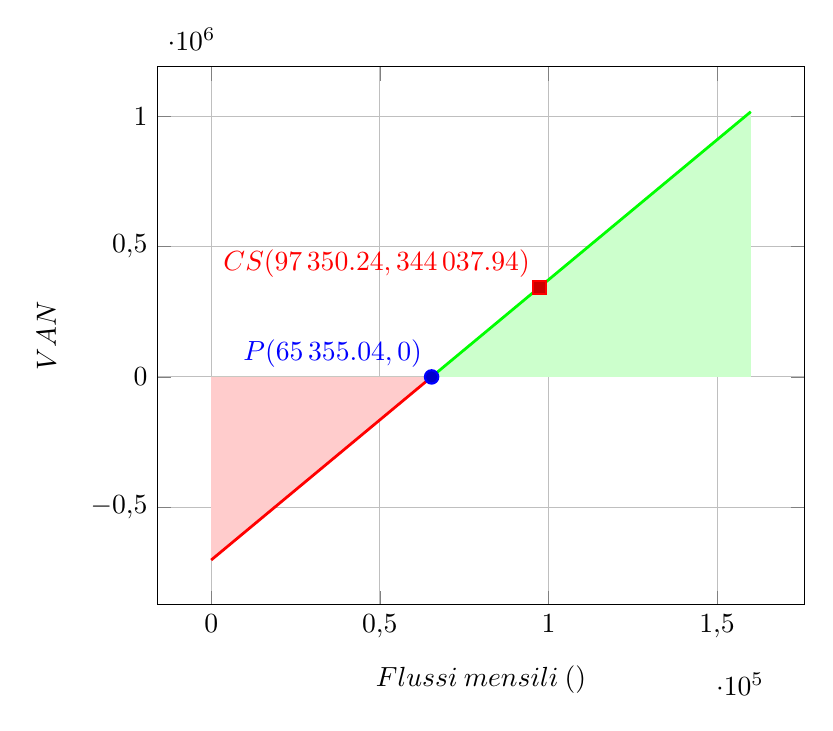
\begin{tikzpicture}[scale=1.2]
 \pgfkeys {
			/pgf/number format/.cd,
			set decimal separator={,{\!}},
			set thousands separator={}}

    \begin{axis}[thick,smooth, xlabel=$Flussi \: mensili \:(\mbox{\euro})$, ylabel=$VAN$, grid=major]    

		\addplot coordinates{( 65355.04, 0) };
		\addplot coordinates{( 97350.24, 344037.94) };

        \coordinate[label=above left:\textcolor{blue}{$ P(65\thinspace 355.04,0)$}](a) at (65355.04,0);
        \coordinate[label=above left:\textcolor{red}{$ CS(97\thinspace 350.24,344\thinspace037.94)$}](a) at (97350.24,344037.94);        
							  
        \addplot+[domain=0:65355.04, name path=A,red,line width=1pt, no markers] {10.7528 * x - 702749.72};
        \addplot+[domain=65355.04:160000, name path=C,green,line width=1pt, no markers] {10.7528 * x - 702749.72};
        \addplot+[domain=0:160000, name path=B, draw=none,black, no markers] {0};

        \addplot[domain=0:65355.04, red!20] fill between[of=A and B];
        \addplot[domain=65355.04:160000, green!20] fill between[of=C and B];
    \end{axis}
\end{tikzpicture}

Considerando il fatturato mensile pari a $\mbox{\euro \: 97\thinspace 350,24}$, gli utili saranno pari a:
	\begin{equation}
	\label{eq:flussi_netti}
	\begin{split}
 		97\thinspace 350,24 \: \mbox{\euro} - \underbrace{60\thinspace 131,27 \: \mbox{\euro}}_{OPEX} = 37\thinspace 218,97 \: \mbox{\euro}	
 	\end{split}
	\end{equation}
fissando il tasso di sconto pari a (\ref{eq:wacc_tax_value}), si può osservare la seguente situazione:
%
%	Tabella relativa alla valutazione VAN = 0,00
%
\begin{savenotes}
\begin{table}[htb]
\centering
 \caption{VAN (Fatturato Mensile pari a $\mbox{\euro \:97\thinspace 350,24}$)}
 \begin{tabular}{p{5cm}D{,}{,}{7.2}D{,}{,}{7.2}D{,}{,}{7.2}}
 \toprule
 	\multicolumn{1}{c}{\textbf{Mese}} & \multicolumn{3}{c}{\textbf{Flussi di cassa (\euro)}} \\
 	& \multicolumn{1}{c}{Netti (\euro)} & \multicolumn{1}{c}{Attualizzati (\euro)} & \multicolumn{1}{c}{Totale (\euro)} \\
 \midrule
 	\makebox[5cm][r]{\textbf{Investimento Iniziale (CAPEX)}} & & & -56\thinspace 170,20 \\
 \midrule
 	\makebox[5cm][r]{Gennaio} & 37\thinspace 218,95 & 36\thinspace 586,00 & -19\thinspace 584,20\\ 
 	\makebox[5cm][r]{Febbraio} & 37\thinspace 218,95 & 35\thinspace 963,83 & 16\thinspace 379,63\\
 	\makebox[5cm][r]{Marzo} & 37\thinspace 218,95 & 35\thinspace 352,23 & 51\thinspace 731,86\\ 
 	\makebox[5cm][r]{Aprile} & 37\thinspace 218,95 & 34\thinspace 751,04 & 86\thinspace 482,91\\
 	\makebox[5cm][r]{Maggio} & 37\thinspace 218,95 & 34\thinspace 160,07 & 120\thinspace 642,98\\ 
 	\makebox[5cm][r]{Giugno} & 37\thinspace 218,95 & 33\thinspace 579,15 & 154\thinspace 222,13\\
 	\makebox[5cm][r]{Luglio} & 37\thinspace 218,95 & 33\thinspace 008,11 & 187\thinspace 230,24\\ 
 	\makebox[5cm][r]{Agosto} & 37\thinspace 218,95 & 32\thinspace 446,78 & 219\thinspace 677,03\\
 	\makebox[5cm][r]{Settembre} & 37\thinspace 218,95 & 31\thinspace 895,00 & 251\thinspace 572,03\\ 
 	\makebox[5cm][r]{Ottobre} & 37\thinspace 218,95 & 31\thinspace 352,60 & 282\thinspace 924,62\\
 	\makebox[5cm][r]{Novembre} & 37\thinspace 218,95 & 30\thinspace 819,42 & 313\thinspace 744,05\\ 
 	\makebox[5cm][r]{Dicembre} & 37\thinspace 218,95 & 30\thinspace 295,31 & 344\thinspace 039,36\\ 
 \bottomrule
 \end{tabular} 
\end{table}
\end{savenotes}
quindi si può osservare come già nel mese di Febbraio riusciamo ad avere il \textbf{pareggio} con l'investimento iniziale!